% !TEX root = ../intro-stellar-physics.tex

\section{The Boltzmann Equation}
\label{s.boltzmann-eqn}

Suppose we have a sample of atoms, all of the same species.  The electrons in those atoms can be in any number of energy levels; we'll denote the energy of level $n$ as $E_{n}$.  There may be many different states with the same energy; we'll denote the total number of possible states\sidenote{Known as the \emph{degeneracy} of a given energy} with energy $E_{n}$ as $g_{n}$.  For example, in a neutral hydrogen atom, the energy and degeneracy of level $n$ are
\begin{eqnarray*}
 E_{n} &=& \val{13.6}{\eV}\left(1-\frac{1}{n^{2}}\right)\\
 g_{n} &=& 2n^{2}.
\end{eqnarray*}
Here the ground state has $n = 1$ and $E_{1} = \val{0}{\eV}$.

The basic principle of statistical (thermal) physics is that if our sample is in thermal equilibrium, then the ratio of the number of atoms in state $i$ to the number in state $j$ is
\begin{equation}\label{e.boltzmann}
\frac{N_{i}}{N_{j}} = \frac{g_{i}}{g_{j}} 
\exp\left(-\frac{E_{i}-E_{j}}{\kB T}\right).
\end{equation}
Suppose we wish to know the fraction of atoms in a given state $i$: that is, we want to know
\[	x_{i} = \frac{N_{i}}{N_{1}+N_{2}+\ldots+N_{i}+\ldots} ? \]
Using equation~(\ref{e.boltzmann}), we can express $x_{i}$ as 
\begin{eqnarray}
  x_{i} &=& \frac{N_{i}/N_{1}}{1+N_{2}/N_{1}+\ldots+N_{i}/N_{1}+\ldots}\nonumber\\
        &=& \frac{g_{i}e^{-E_{i}/\kB T}}{g_{1}e^{-E_{1}/\kB T}+g_{2}e^{-E_{2}/\kB T}+\ldots+g_{i}e^{-E_{i}/\kB T}+\ldots} \nonumber\\
        &\equiv& \frac{g_{i}e^{-E_{i}/\kB T}}{\pfcn}.
\end{eqnarray}
The quantity 
\[ \pfcn = \sum_{i} g_{i}\exp\left(-\frac{E_{i}}{\kB T}\right) \]
is called the \emph{partition function}: loosely speaking, it indicates the number of ways the sample of atoms can be partitioned among the different energy levels.

\begin{exercisebox}[Partition function for neutral hydrogen]
For a neutral hydrogen atom, what is the limit of $\pfcn_{\mathrm{H}}(T)$ for $\kB T \ll \val{13.6}{\eV}$?  How does $\pfcn_{\mathrm{H}}(T)$ qualitatively change with temperature: does it increase, decrease, or something else?
\end{exercisebox}

\section{Ionization: The Saha equation}
\label{s.saha-eqn}

As the temperature in the gas rises, collisions between atoms become sufficiently energetic to eject electrons from atoms.  In astronomy, the ionization state is denoted by a small Roman numeral: Fe\,\textsc{i} denotes neutral iron, Fe\,\textsc{ii} denotes singly-ionized iron, Fe\,\textsc{iii} denotes doubly-ionized iron, and so on. We'd like to extend equation~(\ref{e.boltzmann}) to find the ratios of two ionization states $N\,(i+1)/N\,(i)$.  There are some complications, however, and deriving this ratio is beyond the scope of this course. What we will do is look at the equation for this ratio, known as the \emph{Saha equation}, and try to understand how it works.  The Saha equation for the ratio of ionized to neutron hydrogen is
\begin{equation}\label{e.saha}
\frac{N\,\textrm{\scshape ii}}{N\,\textrm{\scshape i}} 
= {\color{red}\left[\frac{2}{n_{e}}
\left(\frac{2\pi m_{e}kT}{h^{2}}\right)^{3/2}\right]}
\frac{\pfcn_{\mathrm{II}}}{\pfcn_{\mathrm{I}}} \exp\left(-\frac{E_{\mathrm{ion}}}{\kB T}\right).
\end{equation}
In this equation, $n_{e}$ denotes the electron density---the number of free electrons per unit volume---and $m_{e}$ is the electron mass.

Let us interpret equation~(\ref{e.saha}) in terms of eq.~(\ref{e.boltzmann}).  First, there is the factor $\exp(-E_{\mathrm{ion}}/\kB T)$. Here $E_{\mathrm{ion}}$ is the difference in energy between the ground states of the different ionization stages (for this example, $E_{\mathrm{ion}} = \val{13.6}{\eV}$).  That is just as in equation~(\ref{e.boltzmann}). To understand the factor $\pfcn_{\mathrm{II}}/\pfcn_{\mathrm{I}}$, consider that we are asking for the ratio between the total number of ionized atoms to the total number of neutral atoms; and this means summing over all of the states with electrons in different energy states. It is plausible, therefore, that the factor $g_{i}/g_{j}$ from equation~(\ref{e.boltzmann}) would be replaced by $\pfcn_{\mathrm{II}}/\pfcn_{\mathrm{I}}$.

In addition to the number of possible states for the ion, we need to allow for the number of possible electron states.  When the atom is ionized, each electron quickly acquires an average kinetic energy $(3/2)\kB T$. There are many different states with this energy: the electron can be in different locations, and moving in different directions.  At first, you might think that there would be an infinitude of possible electron states.  Quantum mechanics, however, sets limitations on the number of electron states.

First, we have the Pauli exclusion principle: no two electrons can be in the same location with the same momentum and same spin. What do we mean by same location and momentum?  Recall the Heisenberg uncertainty principle: the electrons $x$-position and $x$-momentum are spread about a range of values $\Delta x$ and $\Delta p_{x}$, and these uncertainties are related via
\[ \Delta x\,\Delta p_{x} \gtrsim h. \]
Thus, if we imagine dividing our volume into little boxes of volume
\[ 
 \Delta V = \Delta x\,\Delta y\,\Delta z \approx \frac{h^{3}}{\Delta p_{x}\,\Delta p_{y}\,\Delta p_{z}},
\]
each box can hold two electrons.\sidenote{Because electrons have spin 1/2, we can put two electrons into the same position and momentum state if their spins are oppositely directed.} Suppose we have a volume $V$; how many boxes are there?  The number of available boxes is
\[
	\frac{V}{\Delta V} \approx \frac{V\;\Delta p_{x}\,\Delta p_{y}\,\Delta p_{z}}{h^{3}}.
\]
To estimate the size of $\Delta p_{x}\,\Delta p_{y}\,\Delta p_{z}$, let's estimate $\Delta p_{x}\sim p_{x}$; further, if everthing is isotropic then $p_{x}\approx p_{y}\approx p_{z}$ on average, so $\Delta p_{x}\,\Delta p_{y}\,\Delta p_{z} \sim p_{x}^{3}$.  Now the kinetic energy of the electron is $p^{2}/2m_{e}$, and $p^{2} = p_{x}^{2} + p_{y}^{2} + p_{z}^{2} \approx 3 p_{x}^{2}$. Hence the kinetic energy is $(3/2)p_{x}^{2}/m_{e}$; in thermal equilibrium, however, the kinetic energy has an average value of $(3/2)\kB T$.  The value of $p_{x}^{2}$ is therefore
\[
	p_{x}^{2} \approx m_{e}\kB T,
\]
and the number of boxes is
\[
	\frac{V}{\Delta V} \sim V\frac{p_{x}^{3}}{h^{3}} \sim V\frac{\left(m_{e}\kB T\right)^{3/2}}{h^{3}}.
\]
If our volume $V$ contains $N_{e}$ electrons, then the number of boxes---which is the number of states---per electron is
\[
	\frac{2V}{N_{e}\Delta V} \sim \frac{2V}{N_{e}}\frac{\left(m_{e}\kB T\right)^{3/2}}{h^{3}}.
\]
The factor of 2 appears because each box can hold 2 electrons.  Recognizing that $N_{e}/V = n_{e}$, we see that this number of states per free electrons corresponds to the factor in $\color{red}\left[\;\right]$ in equation~(\ref{e.saha}). When the numerical calculation is done correctly, the additional factor of $2\pi$ arises.

\section{Mass density and the mean molecular weight}
\label{s.mean-molecular-weight}

It is often useful to refer to the mass density---that is, the mass per unit volume, denoted by $\rho$---rather than the number density.  To compute $\rho$ we multiply the number density of each particle by its mass and sum over all particle species:
\[ \rho = \sum_{i=1}^{N} m_i \, n_i. \]
\newpage
Appendix F in \citetalt{LeBlanc2010An-Introduction} lists the masses of various atoms in units of the atomic mass unit\sidenote{$\val{1}{\amu} = \val{\sci{1.661}{-27}}{\kilo\gram}$ is 1/12 the mass of a neutral \carbon\ atom in its ground state}.  Notice that $m_{e}$ is quite small compared to atomic masses: we can usually ignore $m_{e}$ unless high accuracy is required.  Further note that the mass of an atom, when measured in $\amu$, is quite close to the number of nucleons in that species: $m(\hydrogen)\approx \val{1}{\amu}$; $m(\helium)\approx\val{4}{\amu}$; $m(\oxygen)\approx\val{16}{\amu}$.

It is often convenient to specify $\rho$ in terms of a mean molecular weight $\mu$, defined by
\begin{equation}\label{e.mean-mol-weight}
\frac{\rho}{\mu\mb} = n_{\mathrm{tot}},
\end{equation}
where $\mb$ has a mass of $\val{1}{\amu}$.  From the expressions for $\rho$ and $n_{\mathrm{tot}}$, it follows that
\[
	\mu = \frac{\rho}{\mb n_{\mathrm{tot}}} = \frac{1}{\mb}\frac{\sum_{i}m_{i}\,n_{i}}{\sum_{i}n_{i}}.
\]
For example, in a fully ionized hydrogen gas ($n_{e} = n_{\mathrm{II}}$),
\[
	\mu = \frac{1}{\mb}\frac{m_{e}\,n_{e} + m_{\mathrm{II}}\,n_{\mathrm{II}}}{n_{e}+n_{\mathrm{II}}}
	 \approx \frac{\val{1}{\mb}n_{\mathrm{II}}}{2 \mb n_{\mathrm{II}}} = \frac{1}{2}.
\]
For singly ionized helium ($n_{e} = n_{\mathrm{II}}$), the mean molecular weight is
\[
	\mu = \frac{1}{\mb}\frac{m_{e}\,n_{e} + m_{\mathrm{II}}\,n_{\mathrm{II}}}{n_{e}+n_{\mathrm{II}}}
	 \approx \frac{\val{4}{\mb}n_{\mathrm{II}}}{2 \mb n_{\mathrm{II}}} = 2.
\]
The mean molecular weight is larger because a \helium\ atom is approximately 4 times more massive than a hydrogen atom.

\begin{exercisebox}[Mean molecular weight for ionized helium]
What is $\mu$ for a fully ionized \helium\ gas (2 electrons per atom)? 
\end{exercisebox}

\section{Classifying Stars}

In an influential PhD thesis, \citetalt{Payne1925Stellar-Atmosph} applied the Boltzmann and Saha equations to show that different stellar spectra were consistent with changes in temperature, rather than composition, of the stellar photosphere.  Standard stellar spectra at optical wavelength are shown in Fig.~\ref{f.spectral-types}.  The Balmer lines, which correspond to transitions $2\to3$, $2\to 4$, \ldots, are most prominent in A stars.  These stars have $\Teff = \valrng[--]{7\,500}{9\,500}{\K}$. At lower temperatures, the population of hydrogen atoms in the level $n=2$ decreases as $e^{-E_{2}/kT}$ and the lines become weak.  At higher temperatures, the number of neutral hydrogen atoms decreases; most of the hydrogen is ionized, and the Balmer lines again become weaker.

These arguments apply to other species present in the stellar photosphere.  In the hottest stars (type O: $\Teff > \val{30\,000}{\K}$), hydrogen is mostly ionized and the lines are He\,\textsc{ii} and multiply-ionized metals. As temperature cool into the B and A series, the hydrogen lines increase in strength. Going from F into G ($\Teff = \valrng[--]{5\,000}{6\,000}{\K}$, the hydrogen lines decrease, while lines from singly-ionized and neutral metals such as Ca\,\textsc{ii}, Ca\,\textsc{i}, Fe\,\textsc{i} become strong.  At still lower temperatures in the K and M ($\Teff < \val{3\,500}{\K}$) types, absorption from molecules such as TiO becomes prominant.  An example is the broad trough seen in the K spectrum near $\lambda = \val{500}{\nano\meter}$ in Fig.~\ref{f.spectral-types}.

\begin{figure*}[hb]
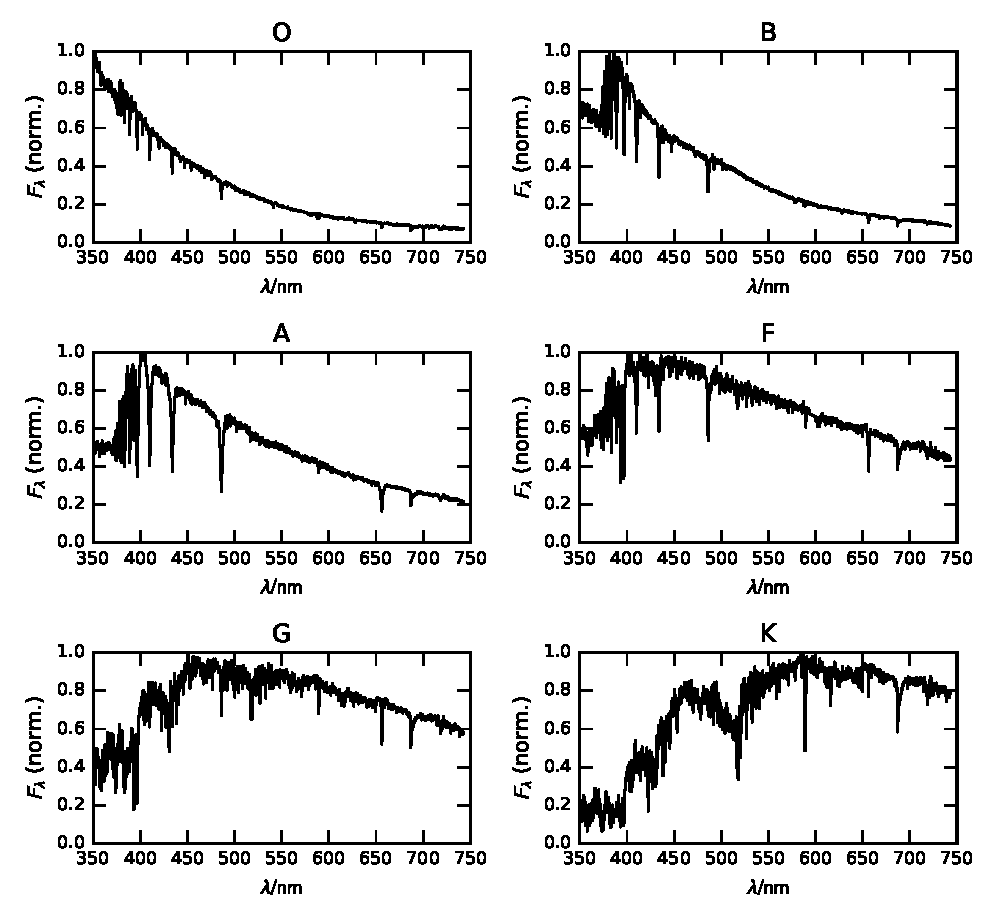
\includegraphics[width=\linewidth]{spectral_types}
\caption[Standard stellar types]{\label{f.spectral-types} Spectra from main-sequence stars of spectral types O--K. Data from \protect\citet{Jacoby1984A-library-of-st}.}
\end{figure*}


\newthought{There is an intrinsic width $\Gamma$ that is set by the finite lifetime of the energy levels;} in practice, however, this is not important.  In a stellar atmosphere, the width $\Gamma$ is set by collisions.  For example, when an electron passes close by our atom, the electric field shifts the energy levels of the atom\sidenote{This is an application of the \emph{Stark} effect that you learn about in quantum mechanics.}.  The greater the collision rate, the larger the width.
If we have two stars of the same photospheric temperature (so that both stars have the same lines), then a way to increase the collision rate is to increase the pressure. Recall, however, that in the stellar atmosphere $P = (g/\kappa)\tau$; as a result, stars with a higher surface gravity will have broader lines. The inset in Figure~\ref{f.compare_grav} illustrates the broadening of the Balmer H$\gamma$ line ($5\to 2$) in the spectrum of a main-sequence A1 star compared with that of a supergiant A1 star.

\begin{figure}[hp]
    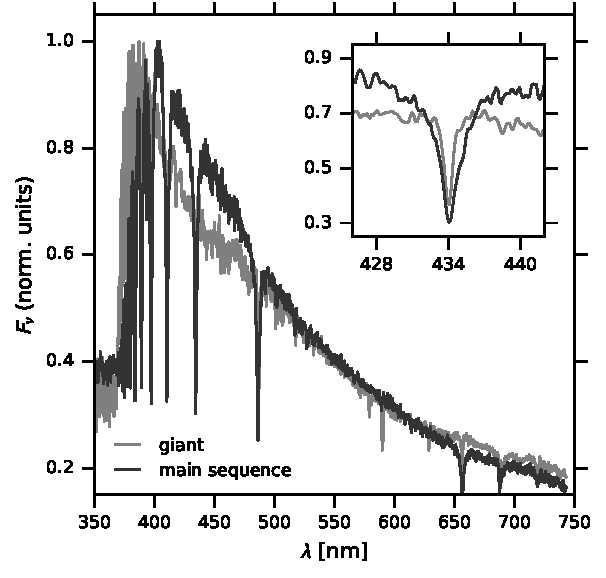
\includegraphics[width=\linewidth]{compare_grav}
    \caption[Spectra of two A1 stars]{\label{f.compare_grav}
    Spectra of two A1 stars, HD 16608 (a main sequence star) and SAO 12149 (a supergiant star).  Spectra are from \citet{Jacoby1984A-library-of-st}.
    }
\end{figure}

In addition to the width set by collisions, the line is also broadened by thermal motion: the atoms are in ceaseless motion; those headed towards us absorb at a blueshifted frequency, while those headed away from us absorb at a redshifted frequency.  Because the atomic velocities follow a Maxwell-Boltzmann distribution, the net effect is to make the core of the line (that is, near the center) assume a Gaussian profile.  Because a Gaussian falls off more quickly than a Lorentzian profile (see Fig.~\ref{f.comparison}), the wings of the line are still determined by the collision rate.

We might be inclined to treat the atoms as hard spheres, but this gives a large $\tau$, or equivalently a narrow line width. We are therefore led to consider longer-range interactions for setting the intrinsic line width. Table~\ref{t.perturbers} lists such interactions. For a given impact parameter, the interaction perturbs the energy levels; by integrating over a distribution of  impact parameters one gets the intrinsic damping. Of course, we should really use a quantum mechanical calculation.  We can scale our cross-section to the classical result (eq.~[\ref{e.cross-section-lorentz}]), however, by writing
\begin{equation}\label{e.cross-section}
	 \sigma_{\nu} = \left(\frac{\pi e^{2}}{m_{e}c}\right) f \phi_{\nu}, 
\end{equation}
where $\phi_{\nu}$ is the line profile (dimension $\sim \Hz^{-1}$) and $f$ is a dimensionless cross-section called the \textbf{oscillator strength}.

\begin{table}[htbp]
\caption{Interactions in stellar atmospheres}\label{t.perturbers}
\begin{tabular}{crcc}
\hline
perturbation & form & source & affects\\
\hline\hline
linear Stark & $C_{2} r^{-2}$ & $e^{-}$, $p$, ions & H (H$\alpha$, H$\beta$, \ldots)\\
quadratic Stark & $C_{4} r^{-4}$ & $e^{-}$ & non-hydrogenic ions\\
van der Waals & $C_{6}r^{-6}$ & atoms, H & most atomic lines, esp.\ in cool stars\\
\hline
\end{tabular}
\end{table}
